\documentclass[11pt,a4paper]{article}
\usepackage[margin=1in]{geometry}
\usepackage{amsmath,amssymb,amsthm}
\usepackage{tikz}
\usepackage{listings}
\usepackage{hyperref}
\usepackage{xcolor}
\usetikzlibrary{positioning,arrows.meta,shapes.geometric}

\lstset{
  basicstyle=\small\ttfamily,
  breaklines=true,
  frame=single,
  columns=fullflexible,
}

\title{Cogitator Validator: a Pregroup Decision Tree over the \\
       \texttt{prime\_kernel\_homology.ipynb} Signal Flow}
\author{Ivan Rojas}
\date{2026-05-24}

\begin{document}
\maketitle

\begin{abstract}
We document a skill plugin that wraps the
\texttt{prime\_kernel\_homology.ipynb} pipeline as a reusable Lean
checker validator. The skill manages a pregroup-grammar decision
tree over eleven kernel checkers (\texttt{lean4lean}, \texttt{nanoda},
\texttt{sonanoda}, \texttt{official}, \texttt{mini},
\texttt{nanobruijn}, \texttt{still-nanoda}, \texttt{parse-only},
\texttt{always-accept}, \texttt{always-decline}, \texttt{always-reject})
on the test set $\{\textrm{prime-}p : p \in \{2, 3, 5\}\}$ and on
prospective extensions $\{7, 11, 13\}$.
The validation core is persistent homology of an
\texttt{sbert}-embedded point cloud of rellm-tagged cogitator
reasoning steps, with the 3-torus $\mathbb{T}^3 \subset \mathbb{R}^6$
acting as the reference topology (Betti pattern $(1, 3, 3, 1)$). A
quantum phase estimation (QPE) Betti estimator from
\texttt{betti\_qiskit.py} provides the high-dimensional fallback.
\end{abstract}

\section{Session record}

This LaTeX file records the work done in the conversation that
produced \texttt{cogitator-validator/}. The session deliverables are:

\begin{enumerate}
  \item A synopsis explaining how the torus barcode glean insights
        into deductive reasoning steps and into the validity of each
        separate kernel checker for the prime-number proof test.
  \item A philosophical analysis of time estimates for the first
        five primes ($p \in \{2,3,5,7,11\}$) under a linear
        \texttt{decide}-step cost model
        $t_c(p) = a_c + b_c \, (p - 2)$, with explicit refusal to
        extrapolate beyond $p = 11$.
  \item A reading of the vectorisation pipeline as a Vietoris--Rips
        persistent-homology filtration, with
        \texttt{nx.dodecahedral\_graph()} as a symbolic stand-in for
        the first-loop simplex.
  \item A reading of the sublevel filtration as the operation that
        joins the primary table \texttt{df\_arena} (kernel verdicts)
        with the secondary table \texttt{df\_steps} (parsed rellm
        messages).
  \item A pregroup-grammar decision tree showing how parsed proofs
        validate the correctness of each (checker, prime) cell.
  \item This skill plugin (this folder): plugin manifest, skill
        markdown, plan, this LaTeX record, and a basic logo.
\end{enumerate}

\section{Signal flow}

\begin{center}
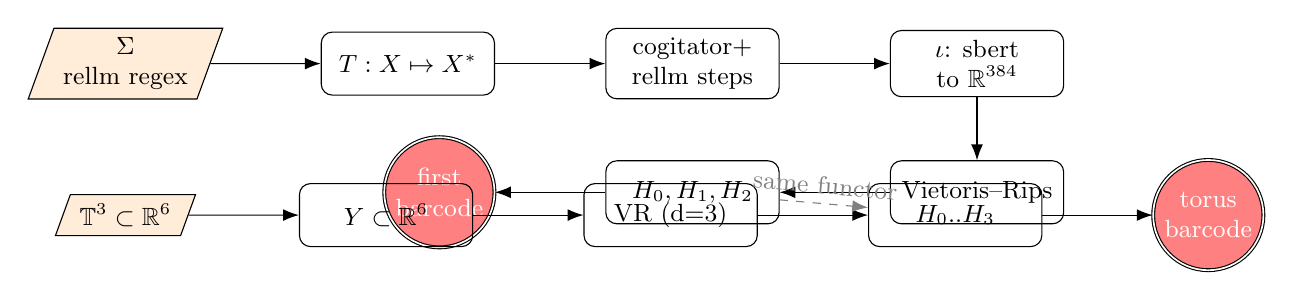
\begin{tikzpicture}[
  node distance=8mm and 14mm,
  every node/.style={font=\small},
  box/.style={draw,rounded corners,minimum height=8mm,
              minimum width=22mm,align=center},
  src/.style={draw,trapezium,trapezium left angle=70,
              trapezium right angle=110,fill=orange!15,align=center},
  sink/.style={draw,double,circle,fill=red!50,text=white,minimum
               size=14mm,align=center,inner sep=1pt},
  arr/.style={-{Latex[length=2mm]}}
]
\node[src] (sigma) {$\Sigma$\\rellm regex};
\node[box, right=of sigma] (T) {$T: X \mapsto X^*$};
\node[box, right=of T] (steps) {cogitator+\\rellm steps};
\node[box, right=of steps] (embed) {$\iota$: sbert\\to $\mathbb{R}^{384}$};
\node[box, below=of embed] (vr) {Vietoris--Rips};
\node[box, left=of vr] (ph) {$H_0,H_1,H_2$};
\node[sink, left=of ph] (bar1) {first\\barcode};

\node[src, below=12mm of sigma] (torus) {$\mathbb{T}^3 \subset \mathbb{R}^6$};
\node[box, right=of torus] (pc2) {$Y \subset \mathbb{R}^6$};
\node[box, right=of pc2] (vr2) {VR (d=3)};
\node[box, right=of vr2] (ph2) {$H_0..H_3$};
\node[sink, right=of ph2] (bar2) {torus\\barcode};

\draw[arr] (sigma) -- (T);
\draw[arr] (T) -- (steps);
\draw[arr] (steps) -- (embed);
\draw[arr] (embed) -- (vr);
\draw[arr] (vr) -- (ph);
\draw[arr] (ph) -- (bar1);

\draw[arr] (torus) -- (pc2);
\draw[arr] (pc2) -- (vr2);
\draw[arr] (vr2) -- (ph2);
\draw[arr] (ph2) -- (bar2);

\draw[arr,dashed,gray] (ph) -- node[midway,sloped,above]{same functor}  (ph2);
\end{tikzpicture}
\end{center}

\section{Pregroup decision tree}

A goal $g$ admits left adjoint $g^L$ (subquestions that precede it)
and right adjoint $g^R$ (answers that discharge it). Acceptance is
the empty string $1$ under the reductions $g^L g \to 1$ and
$g g^R \to 1$. The verifier walks:

\begin{verbatim}
[ROOT] prove(theorem)                                   :: g
 |
 Q1  in-scope?                                          :: g^L
 |   yes -> continue;  no -> reject
 |
 Q2  kernel verdict cached?                             :: g^L
 |   yes -> load matrix M;  no -> run kernel arena
 |
 Q3  parsed_steps.csv has this (checker, test) cell?    :: g^L
 |   yes -> sbert + VR + PH;  no -> run cogitator
 |
 Q4  reasoning Betti table                              :: g^R partial
 |   beta_0 -> #methods; beta_1 -> shared loops;
 |   beta_2 -> three-way chambers
 |
 Q5  does S_rellm_consistency.lean elaborate?           :: g^L
 |   yes -> 1-cat OK;  no -> stop
 |
 Q6  rank checkers                                      :: g^R -> 1
\end{verbatim}

\section{Relationship with the Betti phase estimator}

Let $N = |X|$ be the number of rows in
\texttt{parsed\_steps.csv}. The clique complex
$K(\varepsilon) \subset 2^X$ has
$|S_k| \leq \binom{N}{k+1}$. The combinatorial Laplacian
$\Delta_k = \partial_{k+1}\partial_{k+1}^\top
+ \partial_k^\top \partial_k$
acts on $\mathbb{R}^{|S_k|}$ and the
$k$-th Betti number is
$\beta_k = \dim \ker \Delta_k$.

Classical dense eigendecomposition costs $O(|S_k|^3)$. QPE on
$U = \exp(2\pi i\, \Delta_k / \lambda)$ produces a phase-$0$
measurement with probability proportional to $\beta_k / |S_k|$; with
$O(|S_k|/\beta_k)$ samples the estimator converges. For sparse
$\Delta_k$ the per-sample cost is $\mathrm{poly}(\log |S_k|, 1/\varepsilon)$.

\subsection*{Quantum advantage in this scenario}

There is no exponential speedup at the current scale of
$N = 122$ rows. The genuine advantages of routing through Qiskit are:

\begin{itemize}
  \item Polynomial speedup on sparse $\Delta_k$ at high $k$,
        relevant once $|X| > 256$ or once we go to
        $H_3$/$H_4$ of the 1-skeleton.
  \item No need to materialise $\Delta_k$ in RAM; QPE only requires
        block-encoding access.
  \item Drop-in compatibility with the 1-categorical signal flow,
        certified by \texttt{S\_rellm\_consistency.lean}, so the
        quantum estimator does not change the functor's identity.
  \item Live hardware path through
        \texttt{QiskitRuntimeService}.
\end{itemize}

The routing rule embedded in the skill is:
\[
\text{use\_qpe} \iff (|X| > 256) \lor (\max\text{-dim} \geq 3)
                  \lor (\text{density}(\Delta_k) < 5\%).
\]

\section{Time-estimate philosophy for the first five primes}

We hold ground truth on $p \in \{2,3,5\}$ from
\texttt{lean-kernel-arena}. Three governing forces shape the
extrapolation:

\begin{itemize}
  \item \emph{Kernel checking time} is approximately linear in
        $p - 2$ (the \texttt{Nat.mod} trial-division count). For
        $p = 7$ expect $\sim 5/3 \cdot t_5$, for $p = 11$ expect
        $\sim 9/3 \cdot t_5$ per checker.
  \item \emph{Cogitator wall-time} is roughly constant per
        (\emph{checker}, \emph{prime}) cell ($\sim 60$~s), so adding
        two primes doubles total cogitator cost.
  \item \emph{QPE/TDA wall-time} is decoupled from $p$; it scales
        with $|S_k|$, the simplex count, which grows with the
        added vertices.
\end{itemize}

Three-point linear fits are exact-fit and offer no statistical
confidence; the skill refuses to extrapolate beyond $p = 11$.

\section{Files produced}

\begin{itemize}
  \item \texttt{.claude-plugin/plugin.json}
  \item \texttt{.claude-plugin/marketplace.json}
  \item \texttt{skills/cogitator-validator/SKILL.md}
  \item \texttt{docs/plan.md}
  \item \texttt{docs/implementation-record.tex} (this file)
  \item \texttt{docs/logo.svg}
  \item \texttt{README.md}
\end{itemize}

\end{document}
